\documentclass{article}
\usepackage{tikz}
\usepackage{amsmath}
\usepackage{bm}
\usepackage{scalerel}
\usepackage{pgfplots}
\usepackage{mathpazo}
\pgfplotsset{width=7cm,compat=1.8}
\usetikzlibrary{patterns}
\usetikzlibrary{arrows,shapes,calc}
\usetikzlibrary{external}
\tikzset{external/system call={pdflatex \tikzexternalcheckshellescape -halt-on-error
        -interaction=batchmode -jobname "\image" "\texsource" && %  or ;
pdftops -eps "\image".pdf}}
\tikzexternalize




\begin{document}
	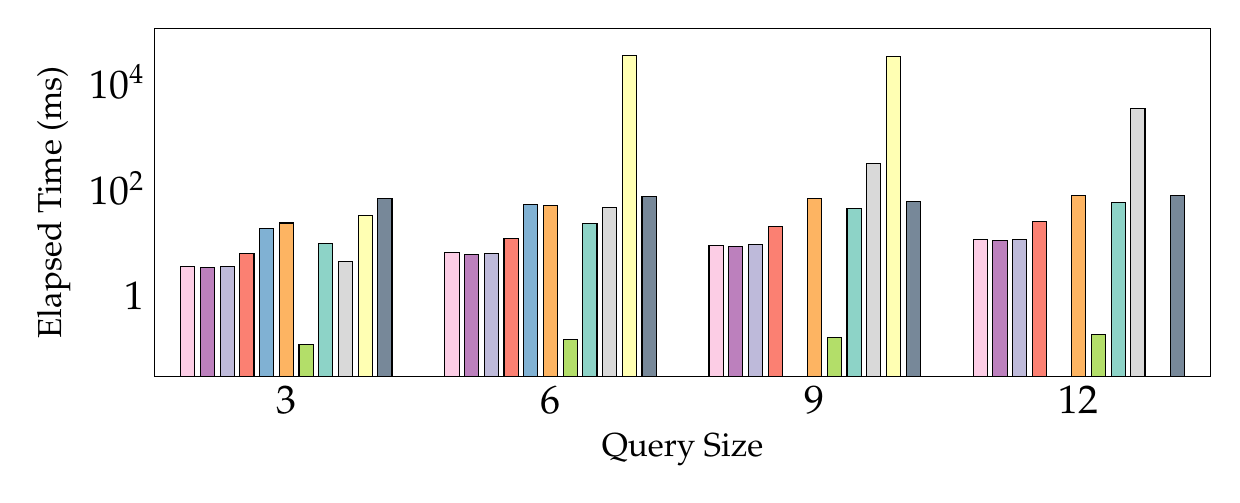
\begin{tikzpicture}
	\definecolor{lssfre}{HTML}{fccde5}
	\definecolor{lssemb}{HTML}{bc80bd}
	\definecolor{lsscon}{HTML}{bebada}
	\definecolor{wj}{HTML}{fb8072}
	\definecolor{impr}{HTML}{80b1d3}
	\definecolor{cs}{HTML}{fdb462}
	\definecolor{cset}{HTML}{b3de69}
	\definecolor{jsub}{HTML}{8dd3c7}
	\definecolor{sumrdf}{HTML}{ffffb3}
	\definecolor{bsk}{HTML}{d9d9d9}
	\definecolor{gflow}{HTML}{778899}
	\centering
	\begin{axis}[
	ybar, %axis on top,
	height=6cm, width=15cm,
	bar width=0.18cm,
	tick align=inside,
	%enlarge y limits={value=.1,upper},
	ymin=0, ymax=100000,
	tickwidth=0pt,
	ymode=log,
	log origin=infty,
	enlarge x limits=true,
	legend style={
		draw=none,
		at={(0.5, 1.3)},
		anchor=north,
		legend columns=1,
		/tikz/every even column/.append style={column sep=0.5cm}
	},
	ylabel={Elapsed Time (ms)},
	ytick={1, 100, 10000},
	yticklabels={$1$,$10^2$, $10^4$},
	xmin=2.5, xmax = 12.5,
	xtick={3,6,9,12},
	xticklabels={3, 6, 9, 12},
	xlabel={Query Size},
	xlabel style={yshift=0ex},
	label style={font=\large},
	tick label style={font=\Large},
	%symbolic x coords={
	%	Facebook, Gowalla, WikiConflict, Google, DBLP, Berkstan, Youtube, Petster, Flickr,
	%Indochina },
	%xtick=data,
	]


	% LSS-fre
 	\addplot [ybar, fill=lssfre, area legend] coordinates {
(3, 3.477689)
(6, 6.241336)
(9, 8.698024)
(12, 11.212315)		
    };
    % LSS-emb
 	\addplot [ybar, fill=lssemb, area legend] coordinates {
(3, 3.369924)
(6, 5.899821)
(9, 8.217740)
(12, 10.463728)	
    };
    % LSS-con
 	\addplot [ybar, fill=lsscon, area legend] coordinates {	
(3, 3.456936)
(6, 6.123104)
(9, 8.772663)
(12, 11.018424)	
    };
    % wj
    \addplot [ybar, fill=wj, area legend] coordinates {
(3, 6.0498)
(6, 11.5358) 
(9, 19.1782)
(12, 24.3602)
    };
    
    % impr
    \addplot [ybar, fill=impr, area legend] coordinates {
(3, 17.8012)
(6, 49.3400)
(9, 0)
(12, 0)
    };
    
    % cs
    \addplot [ybar, fill=cs, area legend] coordinates {
(3, 22.4735)
(6, 47.0279)
(9, 64.1053)
(12, 74.7659)
    };
    
    % cset
    \addplot [ybar, fill=cset, area legend] coordinates {
(3, 0.1195)
(6, 0.1480)
(9, 0.1640)
(12, 0.1859)
    };
    
    % jsub
    \addplot [ybar, fill=jsub, area legend] coordinates {
(3, 9.3909)
(6, 22.1343)
(9, 41.9478)
(12, 53.6647)
    };
    
    % bsk

    \addplot [ybar, fill=bsk, area legend] coordinates {
(3, 4.3265) %
(6, 43.5274)
(9, 297.1492)
(12, 3141.9018)
    };
    
    % sumrdf
    \addplot [ybar, fill=sumrdf, area legend] coordinates {
(3, 30.6625)
(6, 30345.4193)
(9, 29579.9929)
(12, 0)
    };
    
    % gflow
    \addplot [ybar, fill=gflow, area legend] coordinates {
(3, 64.84104893617017)
(6, 71.76215104602507)
(9, 57.773911258278154)
(12, 74.72415609756096)
    };


	
	\legend{
%		    \large $\texttt{LSS-fre}$,
%		    \large $\texttt{LSS-emb}$,
%		    \large $\texttt{LSS-con}$,
%		    \large $\texttt{WJ}$,
%		    \large $\texttt{IMPR}$,
%		    \large $\texttt{CS}$,
%   	    \large $\texttt{CSET}$,
%		    \large $\texttt{JSUB}$,
%		    \large $\texttt{BS}$,
%		    \large $\texttt{SumRDF}$,
%		    \large $\texttt{GFlow}$
	        }
	\end{axis}
	\end{tikzpicture}

\end{document}

